\begin{homeworkProblem}

\textbf{Each of three charged spheres of radius a, one conducting, one having a uniform 
charge density within its volume, and one having a spherically symmetric charge 
density that varies radially as $r^n$ ($n> -3$), has a total charge Q. Use Gauss's theorem 
to obtain the electric fields both inside and outside each sphere. Sketch the behavior 
of the fields as a function of radius for the first two spheres, and for the third with 
n = -2, +2. }

\begin{homeworkSection}{(a)}

Let's break the cases into different problems. The first problem is to find the electric fields over all space for a charge distribution formed by a conducting sphere of radius a. A conductor naturally spreads its static charge uniformly over the surface of the sphere. Thus, no charge resides within the sphere. Gauss' law tells us that $\oint \vec{E}\cdot \vec{da} = \frac{1}{\epsilon_0} \int_{corresponding\;volume} \rho(\vec{r'})d\tau'$. Where $\rho(r')$ is the volume charge density over space. Thus, $\oint_{sphere\;contained\;within\;the\;charged\;sphere} \vec{E} \cdot \vec{da} = 0$. This does not mean, necessarily that the electric field is zero. It only means that the amount of electric field (both negative - entering the surface - and positive - exiting the surface). However, given the symmetry of the problem at hand, all of the electric field lines will point in the radial direction. Thus, $\vec{E}\cdot \vec{da} = E A$, where A is the surface area of the sphere. However, if I were to choose a non-zero volume over which to integrate this dot product (the electric flux) then I would find that A is non-zero. However, in the interior of the sphere, there is no charge. Thus, the electric field must be zero within the interior. Outside of the shell, I have acquired all of the charge. The area of the surface over which I have performed this flux integral is $4\pi r^2$, where r is an arbitrary radius strictly larger than a, the radius of the charged sphere.
\\
Now, $\vec{E}(\vec{r})= \frac{Q}{4\pi a^2 \epsilon_0} \hat{r} H(|\vec{r}|-a)$. The Heaviside step function ``turns on'' my electric field only once my distance away from the origin, r, becomes greater than a.

Sketching this as a function of $|\vec{r}|$, I obtain the following result shown in figure \ref{chargedconductor}. In this figure I have allowed $\frac{Q}{4\pi \epsilon_0} = 1$. The horizontal axis is given in terms of $r/a$.

\begin{figure}%
\centerline{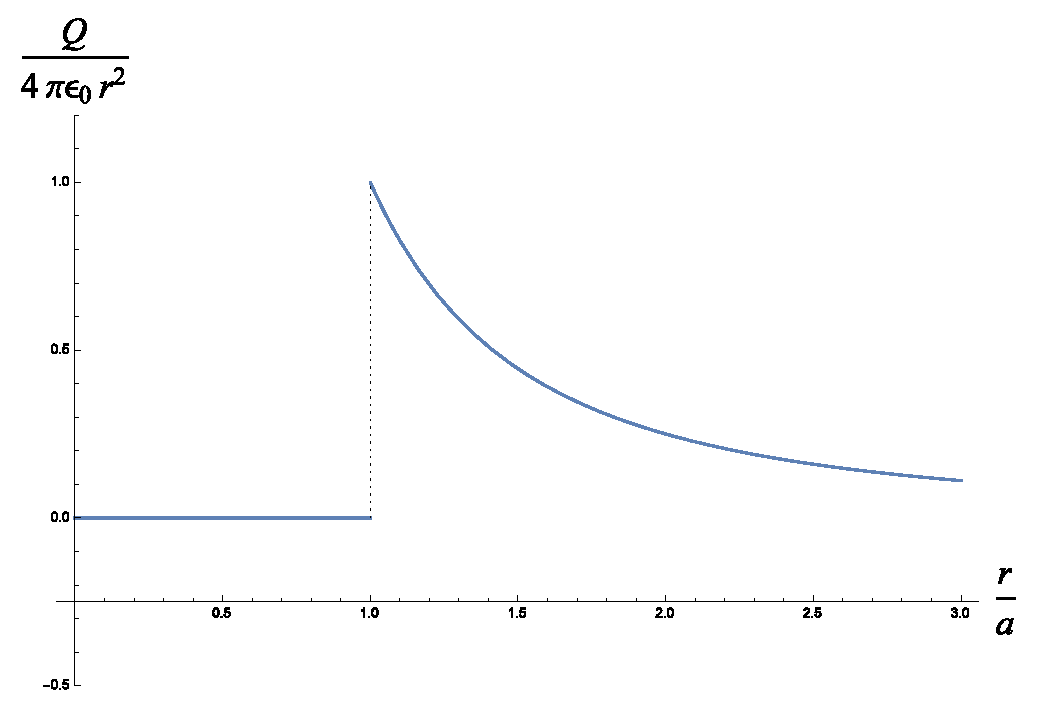
\includegraphics[width=.65\columnwidth,height=.25\paperheight]{./Images/chargedconductor.eps}}%
\caption{Magnitude of the electric field for a charged conducting sphere.}%
\label{chargedconductor}%
\end{figure}

\end{homeworkSection}

\begin{homeworkSection}{(b)}

I must attack the same problem where, now, the charge density is uniform within the volume. Now, as I integrate over the volume of the sphere I acquire charge. But, by symmetry considerations I still have a radial electric field distribution. Thus, $\oint_{area} \vec{E}\cdot \vec{da} = \frac{1}{\epsilon_0} \int_{vol} \rho(r')d\tau'$. The left hand side evaluates to $E(r) 4\pi r^2 = \rho * \frac{4}{3 \epsilon_0}\pi r^3$. This simplifies to $E(r) = \frac{\rho r}{3 \epsilon_0}$. This holds until I get outside of the charged sphere. Then, I have contained all of the charge $Q = \rho * \frac{4\pi a^3}{3}$. Thus, $E(r>a) = \frac{4\pi a^3}{3\epsilon_0} \rho \frac{1}{4\pi r^2} = \frac{\rho a^3}{3\epsilon_0 r^2}$. As a function of $|\vec{r}|$, then, the electric field grows linearly until r = a. Then, the field drops off inverse quadratically. This is plotted in figure \ref{uniformsphere}. The axes and constants have been similarly scaled.

\begin{figure}%
\centerline{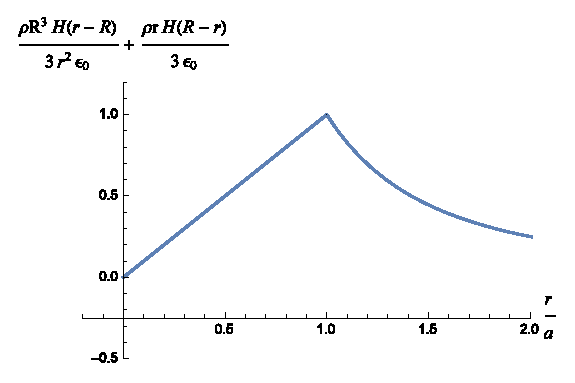
\includegraphics[width=.65\columnwidth,height=.25\paperheight]{./Images/uniformsphere.eps}}%
\caption{Magnitude of the electric field for a uniformly charged sphere.}%
\label{uniformsphere}%
\end{figure}

\end{homeworkSection}

\begin{homeworkSection}{(c)}

I must now obtain the charge distribution for a nonuniform charge distribution. I have been told that the charge density varies as $r^n$. This implies that $\rho(r)\; \alpha \; r^n H(a-|\vec{r}|)$ or that $\rho(r) = C r^n H(a-|\vec{r}|)$, where C is a normalization constant. C is constrained by the fact that $\int_{all space} \rho(r')d\tau' = Q = 4\pi C \frac{a^{n+3}}{n+3}$. Thus, $C = \frac{Q (n+3)}{4\pi a^3 a^n}$. Identifying $\frac{Q}{4\pi a^3}$ as a sort of volume density, I will assign it the label $\rho_0$. Thus, $\rho(r) = \rho_0 \frac{n+3}{a^n} r^n$; the units work. Now, skipping some algebra $E_n(r) 4\pi r^2 = \rho_0 \frac{n+3}{a^n} \frac{r^{n+3}}{n+3} 4\pi$. So, $E(r) = \rho_0 \frac{n+3}{a^n} \frac{r^{n+1}}{n+3}$. This holds until $r \rightarrow a$ at the radius of the sphere. After that point, the sphere looks like a point charge. So, the field will drop off inverse quadratically.
\\ \par
When n=2, $E_2(r<a) =  \rho_0 \frac{5}{a^5} \frac{r^{3}}{8}$. For n = -2, $E_{-2}(r<a)=\rho_0 \frac{1}{a^-3} r^{-1}$. Thus, for n=2, the field rises cubically until the boundary, then it decays quadratically. For n=-2, the field drops as inverse r until the boundary. Then, it drops off quadratically. The plots for $E_2(r)$ and $E_{-2}(r)$ are given in figures \ref{nistwo} and \ref{nisminustwo}, respetively. Similar scaling has been applied.


\begin{figure}%
\centerline{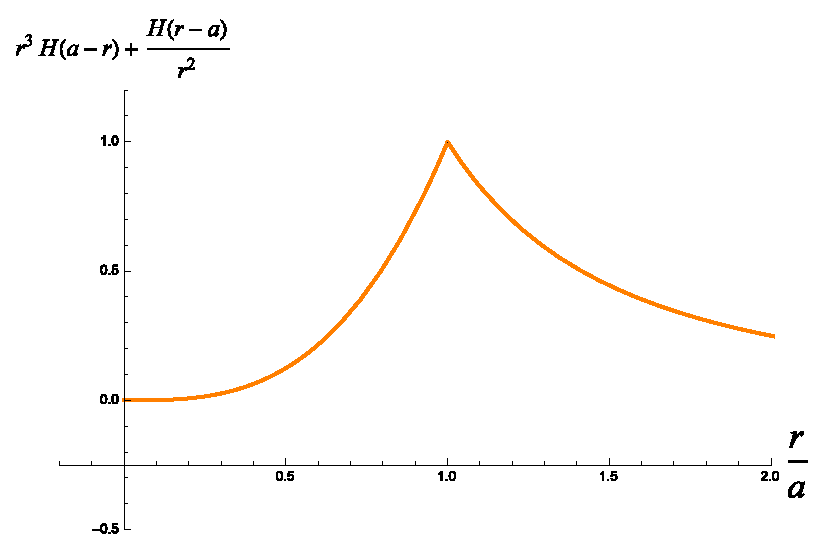
\includegraphics[width=.65\columnwidth,height=.25\paperheight]{./Images/nsphereequalstwo.eps}}%
\caption{Magnitude of the electric field for a charged sphere whose volume charge density varies as $r^2$.}%
\label{nistwo}%
\end{figure}


\begin{figure}%
\centerline{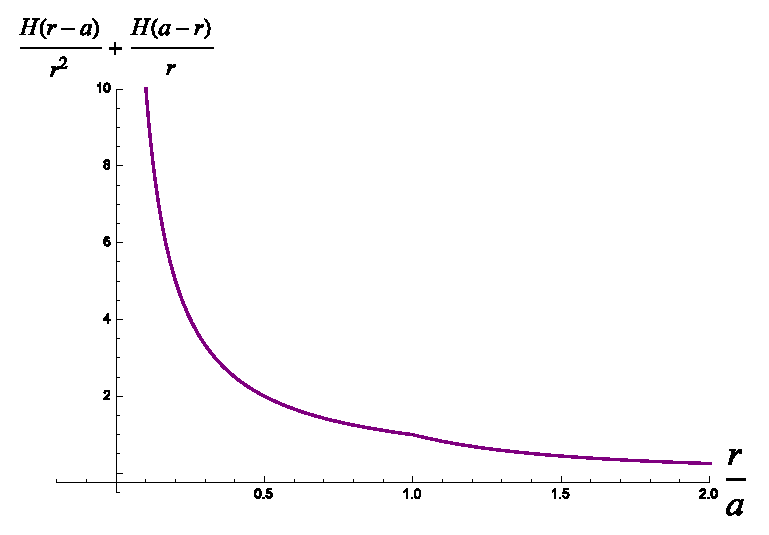
\includegraphics[width=.65\columnwidth,height=.25\paperheight]{./Images/nsphereequalsminustwo.eps}}%
\caption{Magnitude of the electric field for a charged sphere whose volume charge density varies as $r^-2$.}%
\label{nisminustwo}%
\end{figure}

\end{homeworkSection}

\end{homeworkProblem}

